\section{FITT-rammeverket}
\label{sec:fitt-rammeverket}

FITT-rammeverket\footnote{Fit between Individuals, Task and Technology} er et system for å lettere kunne analysere og identifisere de sosiotekniske faktorene som påvirker innføring av nye IT-applikasjoner og -systemer, og dermed kunne peke på hvilke faktorer det er som hinderer en optimal utnyttelse av systemet. Rammeverket er bekrevet i sin helhet i \citep{FITT}.

\noindent
Rammeverket deler settingen IT-systemet skal brukes i inn i tre objekter (se figur \ref{FITT-arkitekturen}); (1) $"$Individ$"$, det vil si enkeltbrukere eller brukergrupper av systemet og de som utfører alle oppgaver på arbeidsplassen. (2) $"$Oppgave$"$ er helheten av oppgaver og arbeidsprosesser som må utføres av brukeren med den gitte teknologien. (3) $"$Teknologi$"$, som er det tekniske systemet (program- og maskinvare og nettverk) og andre verktøy som individene bruker for å utføre oppgavene, inkludert papir-verktøy.
$"$Organisasjon$"$ blir ikke behandlet som et eget objekt i denne sammenhengen, men kan sees som en del av enten bruker-objektet (i betydningen at brukerene jobber i forskjellige roller og grupper i en organisasjon) eller oppgave-objektet (i betydningen at oppgavene og prosessene er organisert på en gitt måte).

\noindent
De tre objektene innehar forskjellige egenskaper, som kan være tilstede i større eller mindre grad. For et individ kan disse være IT-kunnskap, motivasjon og interesse for oppgaven som skal utføres, fleksibilitet og åpenhet for endringer i arbeidsmåte, team-kultur, organisatorisk kontekst, sammarbeidet innenfor team og politikk i en organisasjon. For en oppgave kan det være organisering av oppgavene som skal gjennomføres, gjensidig avhengighet mellom oppgavene og oppgavenes grad av kompleksitet. Teknologien kan ha egnskapene stabilitet og brukbarhet, verktøyets kostnad, funksjonalitet, tilgjengelig teknisk infrastruktur, integrasjon av verktøy og verktøy tilgjengelig i en gitt klinisk situasjon. Dette er ikke fullstendige lister, men kan likevel gi en forståelse for hva slags egenskaper de tre objektene kan ha.

\begin{figure}[H]
\centering
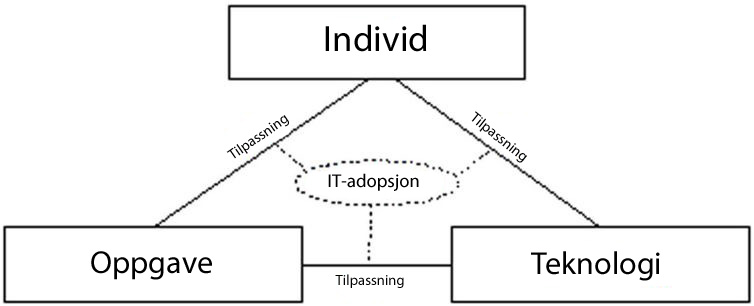
\includegraphics[scale=0.4]{FITT_norsk.jpg}
\caption{FITT-arkitekturen (fritt oversatt av forfatterene. Orginalen kan sees i \citep{FITT})}
\label{FITT-arkitekturen}
\end{figure}

\noindent
Videre ser rammeverket på hvordan disse objektene med sine egnskaper passer (fit) sammen, og sammspillet mellom dem.

Fokuset for rammeverket er samspillet mellom objektene (og deres egenskaper), hvordan de passer (fit) sammen, og ikke objektene i seg selv. Med denne tilnærmingen kan vi definere målet med IT-ledelse som det å finne en optimal tilpassning (fit) mellom bruker, oppgave og teknologi. Dersom objektene mangler, eller har lite utviklede egenskaper som er nødvendig for et optimalt samspill kan man direkte påvirke egenskapene til det enkelte objektet. Et eksempel er ingen eller dårlig IT-kunnskap hos brukerene (individ), hvor opplæring av ansatte kan øke tilstedeværelsen av denne egenskapen. Siden dette er tiltak som påvirker objektene direkte, vil vi kunne si at det er en indirekte påvirkning på samspillet mellom dem.

\noindent
Det vil selvfølgelig alltid finnes eksterne faktorer som er vanskelig eller umulig å påvirke, som høy turnover, eller nye lover og regler. Disse faktorene fører til at det aldri vil oppstå en statisk situasjon med hensyn på de tre dimensjonene av samspill, og derfor heller ikke optimaliseringen av disse.

\noindent
Ved å bruke dette rammeverket kan man lettere se hvor eventuelle problemer ved innføringen av systemet ligger. En vanlig feiltolkning er at problemer som ligger i samspillet mellom bruker og oppgave blir tillagt teknologien. Et eksempel på dette er dersom innføringen av et nytt IT-system gir brukerne større mengde dokumentasjonsoppgaver. Ofte vil det nye systemet (teknologien) få skylden for dette, mens problemet ligger i brukerens misnøye med oppgaven, og ikke har noe med teknologien å gjøre.

